\chapter{Conjugation Table}

Rendering verb forms is a formidable task for new students because there are many things to remember, as well as to know how to put them together. Having a good tool that can provide a good number of examples can speed up the learning process. Unlike a declension table that can be created upon any declinable word, a conjugation table cannot be created for any root due to the lack of complete uniformity.

With this variety of verb formation, we can do, at best, only by providing some typical verb samples, as shown in the left-sided list. And only a handful of verbs have wide range of forms covering most of tenses and moods, for example, \pali{pacati (paca), gacchati (gamu),} and \pali{bhavati (bhū)}. That is why the program starts with \pali{pacati}.\footnote{Rendering \pali{paca} is straightforward and clean, having no weird variations. It may be the most used example for teaching verb formation.}

There are two main modes in this tool: main and derivation. Main verb formation is about \pali{ākhyāta}. So, conjugation makes sense only for main verb forms. Derivative verbs have no conjugation, because they undergo different rules resulting in different verb forms. Most of derivative verbs are declinable. So, we will see declension tables as a result of derivation mode.

Like declension tables, we can check the words rendered against a term list (indexed by Lucene Finder, see Chapter \ref{chap:lister}) by opening the right pane ({\faSix \symbol{"F03A}} button). Opening the right pane can make rendering a new verb sluggish, so use it when necessary.

Rendering a conjugation table has additional two options ({\faSix \symbol{"F560}} button): (1) whether \pali{Attanopada} (middle voice) will be shown, (2) whether Augment (\pali{a-})\footnote{Augment is added only to some of Imperfect verbs and all of Aorist, and Conditional verbs. The augment has no specific meaning, so it is a redundant part. However, it is fashionable to be used with some verbs.} will be added. Figure \ref{fig:conjugation-main} shows aorist forms of \pali{pacati} in full options.

\begin{figure}[!hbt]
\centering
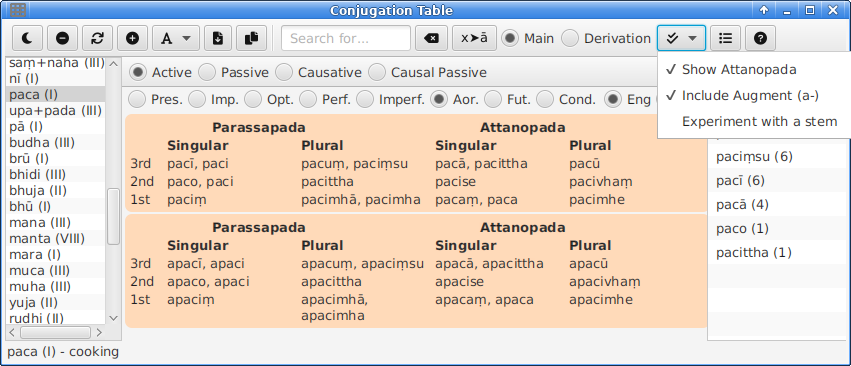
\includegraphics[width=0.9\linewidth]{images/conjugation-main.png}\\
\caption{Aorist forms of \pali{pacati}}
\label{fig:conjugation-main}
\end{figure}

To help new learners, I add Table \ref{tab:tensemood-eng-pali} to show technical terms used by Pāli textbooks, as abbreviated in the result area. However, for those who are new to Pāli grammar and not familiar with verb formation, just playing around this tool can do little help. So, you should read \emph{Pāli for New Learners}\footnote{\url{bhaddacak.github.io/pnl}}, to understand the main idea about Pāli verb formation first.

\begin{table}[!hbt]
\centering
\caption{Tenses and moods}
\label{tab:tensemood-eng-pali}
\bigskip
\begin{tabular}{l>{\itshape}l} \toprule
\bfseries English & \bfseries\upshape Pāli \\
\midrule
Present tense & Vattamānā \\
Imperative mood & Pañcamī \\
Optative mood & Sattamī \\
Perfect tense & Parokkhā \\
Imperfect tense & Hiyyattanī \\
Aorist tense & Ajjatanī \\
Future tense & Bhavissanti \\
Conditional mood & Kālātipatti \\
\bottomrule
\end{tabular}
\end{table}

In Derivation mode, major derivative verb forms can be studied here in various combinations. The result is shown as declension tables, except for \pali{tvā} verbs. Figure \ref{fig:conjugation-deri} show masculine \pali{ta} forms (past participle) of \pali{pacati}. Derivative verbs have substantial details in Pāli grammar, so please see further in the book mentioned.

Like Declension table window, we can experiment with any verb stem here (see the option in {\faSix \symbol{"F560}} button). In experiment mode, the result will be rendered against the generic rules of the verb form selected. This will be useful when the right pane is also opened. In this way, the users can check whether a particular stem has its use in the texts.

\newpage
\begin{figure}[!hbt]
\centering
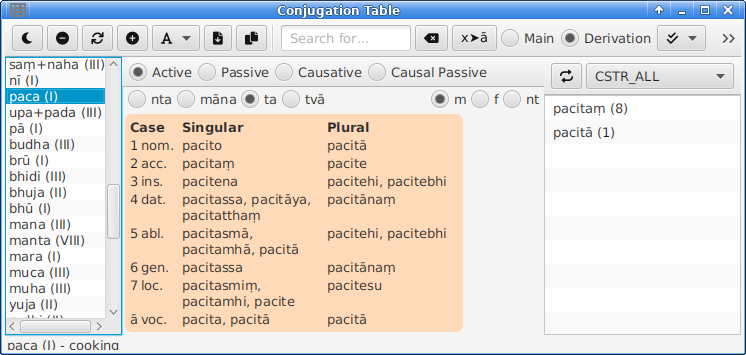
\includegraphics[width=0.9\linewidth]{images/conjugation-deri.png}\\
\caption{Masculine \pali{ta} forms of \pali{pacati}}
\label{fig:conjugation-deri}
\end{figure}
